\documentclass[a4paper, 11pt, twocolumn]{IEEEtran}

\usepackage{graphicx}
\usepackage[scale=.8]{geometry}
\usepackage{microtype}
\usepackage{algpseudocode}
\usepackage{tabularx}
\usepackage{lipsum} 


\title{Some title for a multimodal chess interface}
\author{Giuseppina Iannotti, and Davide Marincione}
\date{11th of June, 2024}

\begin{document}
    \maketitle
    \begin{abstract}
        This is the abstract.
    \end{abstract}

    \section{Introduction}

    {\Huge This intro has to change!}\\
    In this report, we present the design, implementation, and testing, of a multimodal interface for playing chess. The interface allows the user to play with either mouse movements, hand gestures or voice commands. The user can switch between the different modalities at any time during the game. It is implemented in \texttt{python} and uses the \texttt{pygame} library for the audio-visual inteface, \texttt{opencv} and \texttt{mediapipe} for hand gesture recognition, and the \texttt{dragonfly} library for voice commands. The interface has been tested with a group of 12 users, and the results show that the multimodal interface is more engaging and fun to use than a traditional mouse-based interface.

    \section{Coding, Graphics \& Audio}
    \paragraph*{Libraries} A chess program is quite complex to make, and since writing one would've been a project in itself, we have decided to use the \texttt{python-chess} library. This choice enabled us to abstract away the complexity of the game, and to focus on making the interface and the interaction. \texttt{python-chess} is used all over the project's code, to make checks and queries to display the correct information, but also to interact with the chess engine and to make moves.\\For the graphics, audio and event handling, we used the \texttt{pygame} library, which is a set of \texttt{python} modules designed for writing small video games. It is simple yet very powerful, as it allows to draw shapes, images and text on the screen, to play sounds, and to handle user input. Admittedly, it can be quite slow for medium to large-scale projects, as its main drawback is the graphics rendering, which is done via old-fashioned blitting. But, for a project such as ours, it was more than enough.

    \paragraph*{Programming paradigm} For all its usefullness, \texttt{pygame} only provides basic functionalities and none of the data structures and systems used in writing videogames. Things that, to a certain extent, we needed for our project. So we decided to go for an OOP approach, defining ever more refined objects, building on top of more abstract ones. This tactic proved to be extremely successful, as in the later parts of the project there were a couple of instances in which we needed a new class, and we were able to define it without much hassle.
    \begin{figure*}
        \centering
        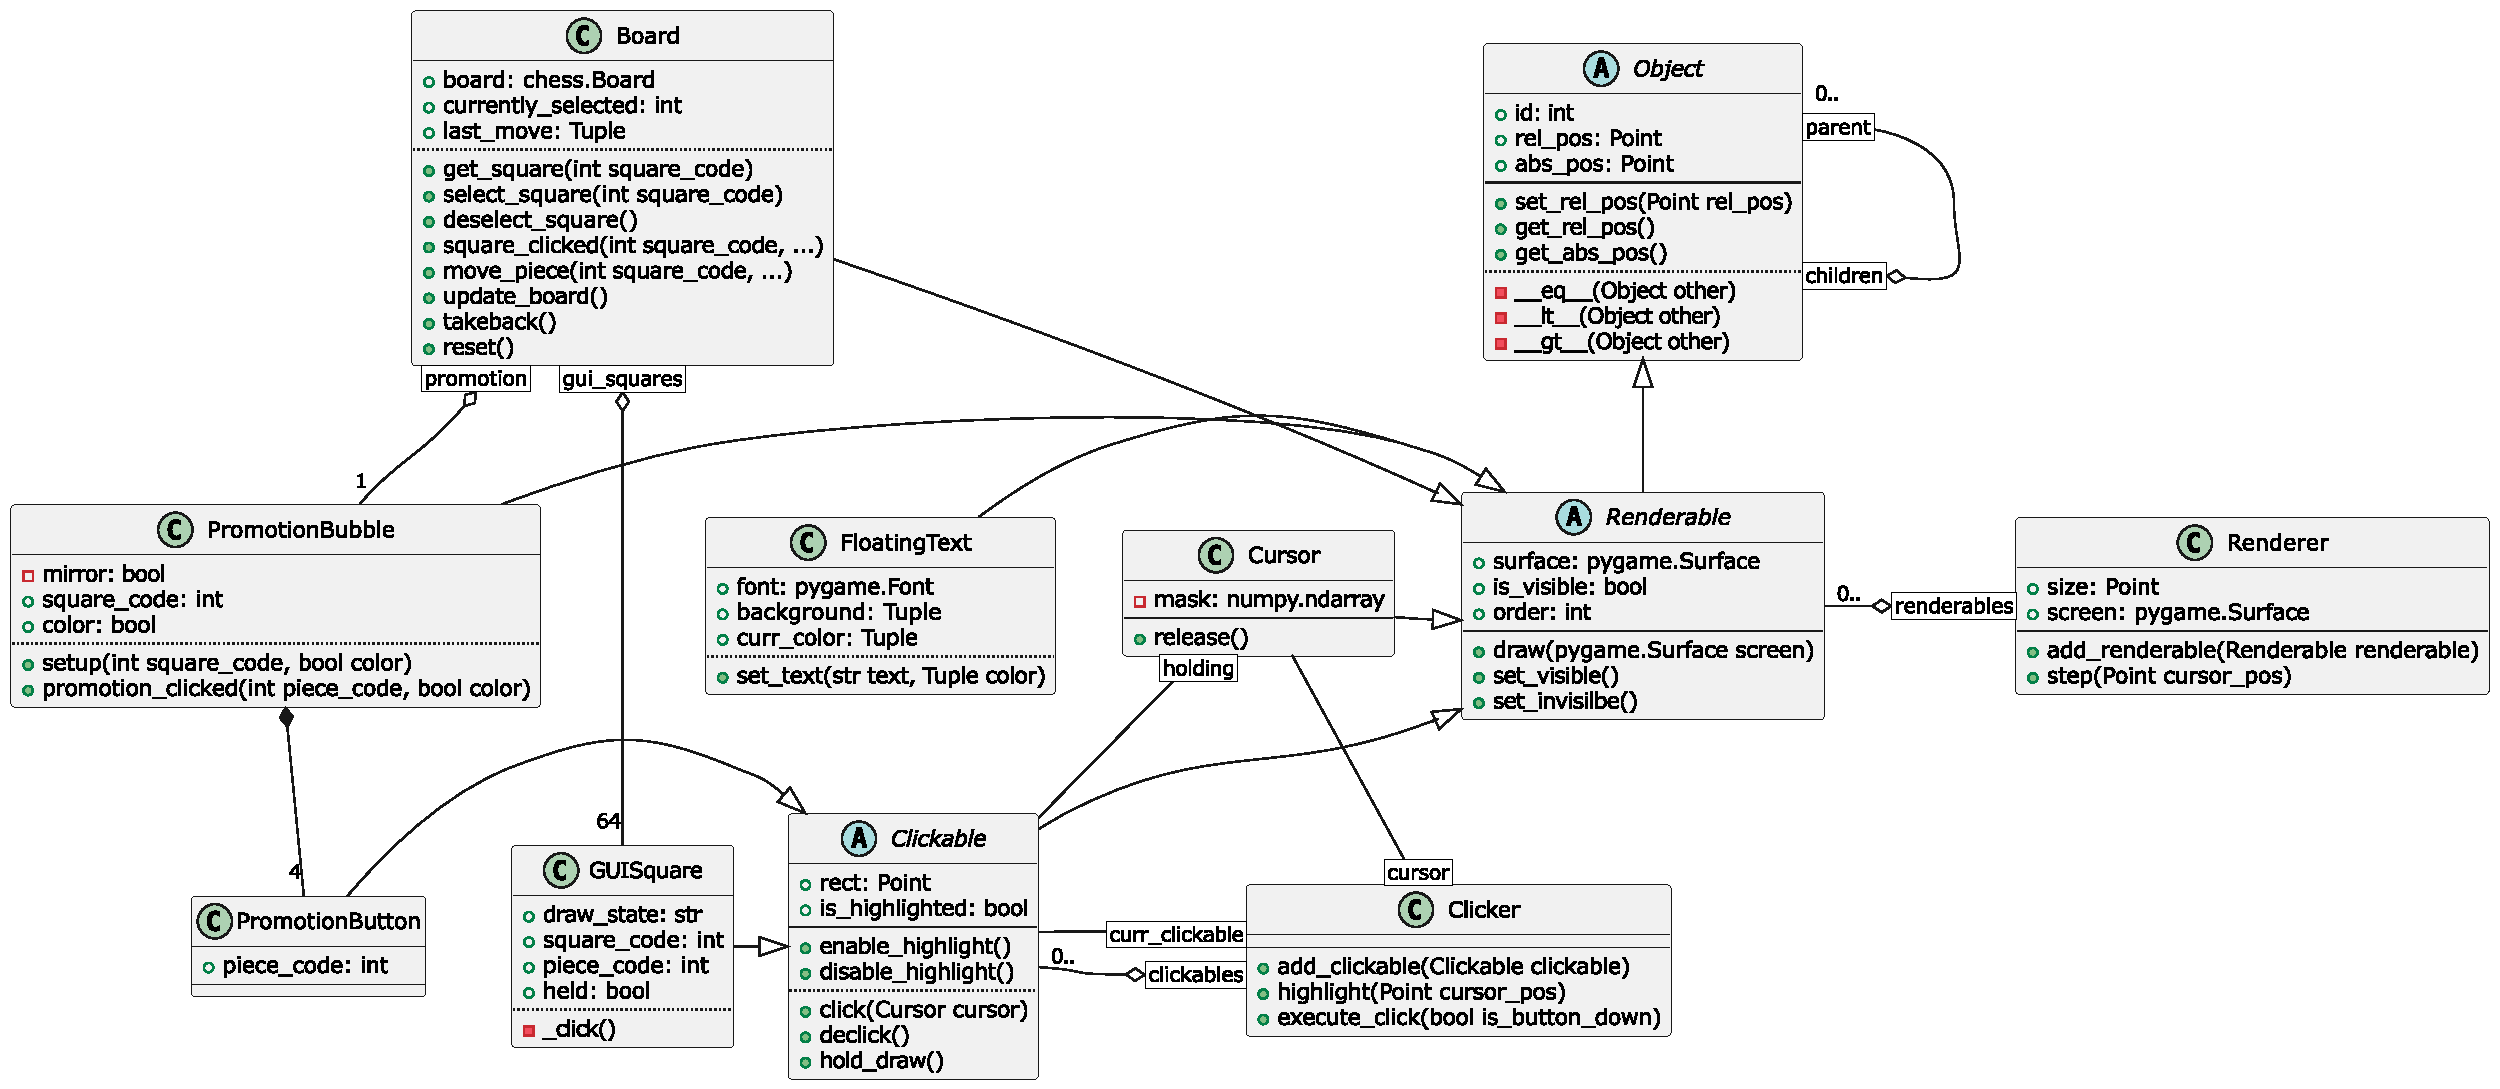
\includegraphics[width=.8\textwidth]{images/uml.pdf}
        \caption{UML description of the basic structure of the program.}
        \label{fig:uml}
    \end{figure*}
    \paragraph*{Basic structure} Inspired by many game engines (Unity, Godot, etc.), our main class is the \texttt{Object} class, which is the base class for most of the elements in our program \ref{fig:uml}. It is defined to be as generic as possible: an object in 2d space which, being in a parent-child hierarchy, can have its absolute position changed by the parent, while maintaining its relative position to it. Internally it has a class-wide \texttt{OBJECT\_COUNTER} member which is used to give each \texttt{Object} its \texttt{id}, used to recognize it among the other objects.
    \paragraph*{Rendering} We then have the \texttt{Renderable} class, which inherits from \texttt{Object}. And, with it, a \texttt{Renderer} class, which is a singleton that keeps track of all the \texttt{Renderable} objects and renders them. As such, the \texttt{Renderable} class has a \texttt{draw()} method, a \texttt{set\_visible()} method and an \texttt{order} attribute, which is used to determine the order in which the objects are rendered. The \texttt{Renderer} class has a \texttt{step()} method, which is called every frame, and it renders all the \texttt{Renderable} objects in the correct order.
    \paragraph*{Clickables} The \texttt{Clickable} class inherits from \texttt{Renderable} and is used to define objects that can be clicked (in our simple system, we don't have invisible but clickable objects). Like with \texttt{Renderer} and \texttt{Renderable}, we have a \texttt{Clicker} singleton, that keeps track of all the \texttt{Clickable}s. It too has a method called every frame, named \texttt{highlight()}, which determines which \texttt{Clickable} would be clicked if a "click" event was called. When that happens, its \texttt{execute\_click()} method is called, which runs the \texttt{click()} and \texttt{declick()}\footnote{The \texttt{declick()} method is run when the left mouse button is released, instead of pressed.} methods that each \texttt{Clickable} must have. This way, we can define different behaviours for different objects.\\Other than that, the \texttt{Clickable} class has a \texttt{enable\_highlight()} method and \texttt{disable\_highlight()} method, which are used to enable and disable the highlight state of the object, respectively. Furthermore, it has a \texttt{hold\_draw()} method, used by the \texttt{Cursor} class to draw the object when it is being held (if it can be held).
    \begin{figure}
        \centering
        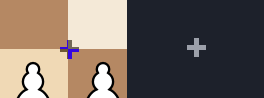
\includegraphics[width=.45\textwidth]{images/cursor_comparison.png}
        \caption{The cursor, with different backgrounds.}
        \label{fig:cursor}
    \end{figure}
    \paragraph*{Cursor} The \texttt{Cursor} class is a singleton that inherits from \texttt{Renderable}. As the name suggests it is used to draw the cursor on the screen, and to keep track of the object that is being held. As described in the next sections it can be driven either by mouse or by hand gestures, and it is referenced by the \texttt{Clicker} as it handles which object is being held (as only \texttt{Clickable}s are holdable). We decided to make the \texttt{Cursor} a \texttt{Renderable} such as to make it different from the os mouse cursor; we felt that it would be better to have a custom cursor such as to give a distinct visual feedback, especially when the cursor is driven by hand gestures. With this class we have made our first interface choice, as the cursor is designed to be a fairly big cross symbol, which distorts the colors it is drawn upon; making it always visible, no matter the background \ref{fig:cursor}. Initially we had thought of using
    \begin{equation}
        c^* = 255 - c,
    \end{equation}
    but we found this to be insufficient, as one can expect most colors to sit in the middle of the color spectrum, thus getting a situation in which the cursor is invisible on most colors, as
    \begin{equation}
        255 - 127 = 128.
    \end{equation}
    To avoid this, we resorted to
    \begin{equation}
        c^* = (c + 128)\ \mathrm{mod}\ 256,
    \end{equation}
    which assures us to always get a color that is distant enough from the original.
    \paragraph*{Text} As we sometimes needed to display text on the screen, we have defined the \texttt{FloatingText} class, which inherits from \texttt{Renderable}. It exploits \texttt{pygame}'s \texttt{Font} class, which is used to render text on the screen, and thanks to that it can dynamically change the displayed text and the color (as the \texttt{Font} class enables that).
    \paragraph*{Board} The \texttt{Board} class is a singleton that inherits from \texttt{Renderable}. Internally, it has a \texttt{board} attribute, which contains a \texttt{chess.Board} object, used to make moves and to check the state of the game. Furthermore, it has a reference to 64 \texttt{GUISquare} objects, which inherit from \texttt{Clickable} and handle the drawing of pieces on the screen, and their interaction with the user. To build a satisfying interface, \texttt{Board} has a number of features:
    \begin{itemize}
        \item It enables a red square under the king when it is in check.
        \item It marks a square with green when it gets selected (as a move can be done by doing two clicks, the first one to select the piece, the second one to select the destination), and highlights in the same way all of the possible moves.
        \item It plays a sound when a move is done, and a different one when a king gets in check.
    \end{itemize}
    \begin{figure}
        \centering
        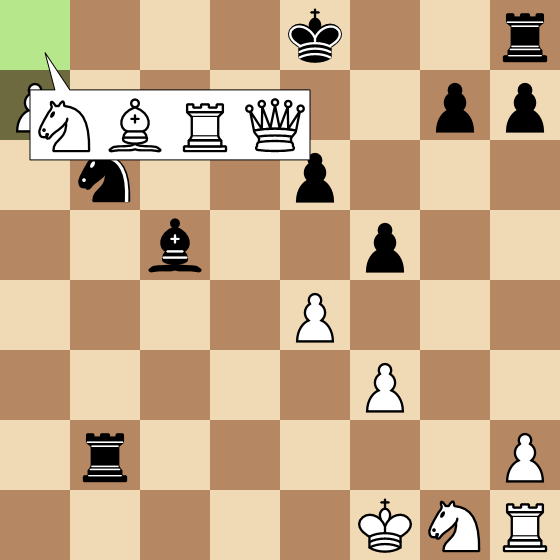
\includegraphics[width=.45\textwidth]{images/promotion_bubble.png}
        \caption{How the promotion bubble looks like.}
        \label{fig:promotion}
    \end{figure}
    \paragraph*{Promotion} The \texttt{Board} recognizes when a pawn reaches the last opposite row, when this happens, before executing the move by calling its internal \texttt{chess.Board} object, it makes a popup element appear, the \texttt{PromotionBubble} \ref{fig:promotion}. This is a \texttt{Renderable} which contains four \texttt{PromotionButton}s, which inherit from \texttt{Clickable}. Each of these buttons represent a piece to which the pawn can be promoted to. When a button is clicked, the \texttt{PromotionBubble} calls the \texttt{Board} to finalize the move and to promote the pawn.
    \paragraph*{Game loop, events and AI} The main loop of the program can be found in \texttt{chess\_main.py}. After the initialization of all the objects and systems, it enters a loop which can be roughly described as follows:
    \begin{enumerate}
        \item Update the cursor position with the latest mouse or hand position, and run \texttt{clicker.highlight(cursor\_pos)}. If a hand gesture is detected, push a mouse event.
        \item Resolve events, such as mouse clicks, key presses (quit game, takebacks), and moves done (for the AI).
        \item Resolve voice commands.
        \item Run \texttt{renderer.step()}.
        \item Run metrics recorder.
    \end{enumerate}
    During the game, the player competes against Stockfish 16 (which, in our tests, we limited); we easily were able to do this thanks to the \texttt{python-chess} library, which has an built-in interface to communicate with a multitude of chess engines. The AI is run during event handling, as our \texttt{Board} emits a custom \texttt{TURN\_DONE} event which we use to discern when the AI has to make a move.
    \paragraph*{Game recording} At the end of development, we wanted to collect quantitative data about the tests. To do this, we implemented a recording system that saves multiple metrics about the runtime; such as the amount of moves made during a modality, the distance traveled with the hand and the number of utterances by the user. In the Experiments section of this report, we'll talk more about this.
    \section{Hand tracking and gestures}
    \paragraph*{Libraries} The hand tracking and gesture recognition system is enabled by the \texttt{opencv} and \texttt{mediapipe} libraries. The first is used to capture the video stream of the camera, and the latter is used to detect and track the hand. The rest of the computation (mapping the hand position to the cursor position, detecting gestures, etc.) is done by our code.
    \paragraph*{Hand detection loop} We design a singleton \texttt{HandDetector} class, which runs its own loop on a separate thread with respect to the main system. This is done to avoid blocking the main loop, and to give as smooth an experience as possible. The loop can be described as follows:
    \begin{enumerate}
        \item Capture the video stream.
        \item If the video stream has stopped, stop the loop.
        \item Flip the video stream horizontally (if needed).
        \item If an async call to the \texttt{mediapipe} library is not running, execute one with the current frame.
    \end{enumerate}
    The async call is done to avoid blocking the loop as the \texttt{mediapipe} library can be quite slow, and the check for no other async calls is done to not accumulate multiple async calls (which, on a slow laptop, can cause the system to crash). Once the async call gets executed, \texttt{mediapipe} runs a custom callback which we design to processes the resulting hand landmarks into the \texttt{Hand} class, which we then store in the \texttt{HandDetector}.
    \paragraph*{Normalizing hands} The landmarks $\mathbf{L}\in\mathrm{R}^3$ that \texttt{mediapipe} produces live in an approximated screen space. This is fairly useful when mapping the hand to the screen space $\mathrm{R}^2$, as we can just disregard the third dimension. But, when one wants to recognize hand gestures while being invariant to different people's hands, it must be modified. Therefore, before storing them, we normalize the landmarks such as to minimize the differences between different hands, their position and orientation.\\
    First and foremost, we extract the palm center $p$ by calculating a weighted average (handmade by us) over the base of the fingers and the wrist
    \begin{equation}
        p = \frac{\mathbf{L}_1}{2} + \frac{\mathbf{L}_6 + \mathbf{L}_{10} + \mathbf{L}_{14} + \mathbf{L}_{18}}{8}.
    \end{equation}
    We extract the palm width $w$, as it is invariant to different hand positions,
    \begin{equation}
        w = ||\mathbf{L}_6 - \mathbf{L}_{18}||_2,
    \end{equation}
    and we get the relative landmarks $\overline{\mathbf{L}}$ by normalizing the landmarks with respect to the palm center and the palm width,
    \begin{equation}
        \overline{\mathbf{L}} = \frac{\mathbf{L} - p}{w}.
    \end{equation}
    \begin{figure}
        \centering
        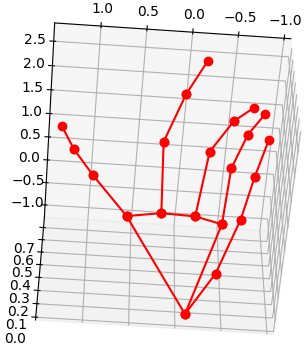
\includegraphics[width=.33\textwidth]{images/norm_hand.png}
        \caption{Right hand in $\mathbf{L}^\star$ doing a grab gesture.}
        \label{fig:norm_hand}
    \end{figure}
    We could've stopped here, as $\overline{\mathbf{L}}$ is enough to recognize the gestures that we designed for the project; but at the time we weren't sure if we would've needed a more expressive representation for more complex gestures. Because of this, we decided to apply a change of basis to $\overline{\mathbf{L}}$ such as to get $\mathbf{L}^\star$, where the internal palm normal is the $z$ axis, the palm width is the $x$ axis (with the positive direction being that of the pinky, regardless of the handedness), and the $y$ axis as their cross product (which, when calculated, should be the direction of the fingers). To do this, we first get the palm normal
    \begin{equation}
        \mathbf{n}_{\mathrm{palm}} = (1 - \mathbf{2}_{\textrm{left}})\frac{(\mathbf{L}_6 - \mathbf{L}_1)\times(\mathbf{L}_{18} - \mathbf{L}_1)}{||(\mathbf{L}_6 - \mathbf{L}_1)\times(\mathbf{L}_{18} - \mathbf{L}_1)||_2},
    \end{equation}
    then we get the pinky normal,
    \begin{equation}
        \mathbf{n}_{\mathrm{pinky}} = (1 - \mathbf{2}_{\textrm{left}})\frac{\mathbf{n}_{\mathrm{palm}}\times(\mathbf{L}_{10} - \mathbf{L}_1)}{||\mathbf{n}_{\mathrm{palm}}\times(\mathbf{L}_{10} - \mathbf{L}_1)||_2}.
    \end{equation}
    and the fingers' normal,
    \begin{equation}
        \mathbf{n}_{\mathrm{fingers}} = (1 - \mathbf{2}_{\textrm{left}})\frac{\mathbf{n}_{\mathrm{pinky}}\times \mathbf{n}_{\mathrm{palm}}}{||\mathbf{n}_{\mathrm{pinky}}\times \mathbf{n}_{\mathrm{palm}}||_2}.
    \end{equation}
    This produces a basis $\mathbf{B} = \left[\mathbf{n}_{\mathrm{pinky}}, \mathbf{n}_{\mathrm{fingers}}, \mathbf{n}_{\mathrm{palm}}\right]$ that is invariant to the hand's orientation, and that gives explicit meaning to the axes. Finally, we produce $\mathbf{L}^\star$,
    \begin{equation}
        \mathbf{L}^\star = \overline{\mathbf{L}}\mathbf{B}^T.
    \end{equation}
    \paragraph*{Gesture recognition} At the outset, we wanted to design two different gestures:
    \begin{enumerate}
        \item A grabbing motion, which would let the user drag-n-drop the pieces. Composed when the thumb and the index are close enough to each other.
        \item A tapping motion, which would let the user click the squares. Composed by a forward flick of the wrist.
    \end{enumerate}
    As we were developing the system, we found that the tapping motion was too hard to recognize reliably (as it doesn't require a change in the landmarks' relative positions). At the same time, we found that the grabbing motion we were developing was actually an already established gesture (used in devices like the Apple Vision Pro) used both for single-click gestures and for drag-n-drop ones. Because of this, we decided to stick with this single gesture, and to use it in a manner akin to pressing the left mouse button.\\
    To recognize the gesture, we design
    \begin{algorithmic}[1]
        \State \textbf{input} \texttt{prev\_click}
        \State $m \gets ||\mathbf{L}^\star_{\mathrm{thumb}} - \mathbf{L}^\star_{\mathrm{index}}||_2$
        \State $d \gets \frac{\mathbf{L}^\star_{\mathrm{thumb}}\cdot\mathbf{L}^\star_{\mathrm{index}}}{||\mathbf{L}^\star_{\mathrm{thumb}}||_2 ||\mathbf{L}^\star_{\mathrm{index}}||_2}$
        \If{\texttt{prev\_click}}
            \State \textbf{return} $m < \alpha_\gamma \land d > \beta_\gamma$
        \Else
            \State \textbf{return} $m < \alpha \land d > \beta$
        \EndIf
    \end{algorithmic}
    where $\alpha$ and $\beta$ are the normal thresholds, and $\alpha_\gamma$ and $\beta_\gamma$ are the thresholds for the hysteresis effect, when the user is already doing a grabbing motion (to avoid dropping the piece when the user is moving it).
    \paragraph*{Hand-cursor mapping} As described in the coding section, at each main loop we retrieve the latest hand-cursor mapping, and, if its timestamp is later than the latest mouse timestamp, we use that. We run the hand-cursor mapping during this main loop, using the latest data given by the hand tracking async code.
    While being fairly precise, \texttt{mediapipe}'s hand tracking system is not perfect: many frames can pass between one detection and the other, tracking is noisy and, finally, the system can lose track of the hand. Therefore we had to build a robust mechanism that could handle these issues.\\
    First and foremost, we use the palm $p$ as the point to map the cursor to, and we rescale and clamp its position to a $[m, M]$ space, such that we can make it easier for the user to reach the edges of the window.
    We do this by
    \begin{equation}
        r = \mathrm{clip}_{[m,M]}(\frac{p - m}{M - m}).
    \end{equation}
    Secondly, we use both the latest position $r_t$ and the previous one $r_{t-1}$ (if these are present, that is). Furthermore, we keep a cursor position $c$ internal to \texttt{HandDetector}, which is independent of the cursor position in the main loop. Then we define an algorithm that updates $c$ and returns it, complete with whether a grab or release event happened (whether the user has started or stopped grabbing).\\
    The algorithm is robust in the sense that it tries to avoid experience-ruining events, such as:
    \begin{enumerate}
        \item The cursor jumping around because of noisy tracking, $c$ moves at a constant rate and can either be updated via bilinear or linear interpolation, based on whether $r_{t-1}$ is present, such as to make its movement smooth (at the cost of being a bit less responsive).
        \item The cursor moving even when the hand is still. This can either happen because humans have a natural tremor in their hands, which can be picked up by the hand tracking system, or because the tracking is noisy. To avoid this, we only update the cursor if the hand has moved a certain distance.
        \item A grabbed piece being dropped for whatever reason, while the user is still keeping a grab gesture. This is avoided by keeping a list of the most recent detections and checking if even one of them is a grab gesture.
    \end{enumerate}
    With all of this combined we achieved a system that, in spite of all the noise and issues, provides a smooth experience. We describe the tests and the results in the Experiments section.

    \section{Voice commands}
    To enhance user interaction with our application, our project aims to integrate voice commands. Playing chess using verbal instructions can provide a more engaging experience and offer advantages over traditional input methods. This approach can be particularly beneficial for users with accessibility needs or those in hands-free environments.
    \paragraph*{Dragonfly} To implement voice commands, we used the \emph{dragonfly} library, a Python package that facilitates the creation of voice command scripts. Dragonfly allows for the intuitive definition of complex command grammars and simplifies the processing of recognition results by treating speech commands and grammar objects as first-class Python objects. Additionally, Dragonfly provides a unified front-end interface that seamlessly integrates with Kaldi as a back-end speech recognition engine.
    
    \begin{table*}[h]
        \centering
        \caption{Rules and Specifications}
        \begin{tabularx}{\textwidth}{|l | X|}
            \hline
            \textbf{Rule Name} & \textbf{Specification} \\
            \hline
            Move Rule & \texttt{"move ( [ <src\_piece>] | [ <src\_piece> [<prep> <src\_square>] to <tgt\_square>] | [ [<prep>] <src\_square> to <tgt\_square>]) [and promote to <prm\_piece>]"} \\
            \hline
            Capture Rule & \texttt{"capture (<tgt\_piece> [<prep> <tgt\_square>] | <tgt\_square>) [with (<src\_piece> [<prep> <src\_square>] | <src\_square>)] [and promote to <prm\_piece>]"}\\
            \hline
            Promote Rule & \texttt{"promote [(<src\_piece> | <src\_square>)] to <prm\_piece>"} \\
            \hline 
            Castle Rule & \texttt{"(castle <special\_direction> | <special\_direction> castle)"} \\
            \hline 
            Piece Rule & \texttt{"<src\_piece> ( [<prep>] <tgt\_square> |in <src\_square> <verb> [<prep>] ( <tgt\_square> | <tgt\_piece> [in <tgt\_square>] ) | <verb> [<prep> <src\_square>]( [<prep>] <tgt\_square> | <tgt\_piece>  [in <tgt\_square>])) [and promote to <prm\_piece>]"}\\
            \hline
            Square Rule & \texttt{"<src\_square> <verb> ( [<prep>] <tgt\_square> | <tgt\_piece> [<prep> <tgt\_square>])"}\\
            \hline
        \end{tabularx}
        \label{tab:rules}
    \end{table*}
    
    
    \paragraph*{Rules} Voice commands are defined using a set of rules that specify the structure of the commands and map them to corresponding actions in the chess game. Each rule is defined as a \texttt{CompoundRule} class, designed to make it very easy to create a rule based on a single compound spec. This rule class has the following parameters to customize its behavior:
    \begin{itemize}
        \item \emph{spec} : Compound specification for the rules root element 
        \item \emph{extras} : Extras elements referenced from the compound spec. It includes choices for prepositions, pieces, and squares.
    \end{itemize}
    The rules are organized into a hierarchy, with each rule defining a specific type of voice command. 
        
    \paragraph*{Grammar} The rules are combined into a grammar object, which is then loaded into the Dragonfly engine. The grammar object is responsible for processing the voice input and matching it against the defined rules. When a match is found, the corresponding action is executed, such as moving a chess piece or promoting a pawn. In particular, our Chess Grammar is composed of the following set of rules, shown at \ref{tab:rules}: 
    \begin{itemize}
        \item \textit{MoveRule}: It defines a structured syntax pattern for recognizing different types of actions, specifically those that start with the verb \emph{"Move"}. Examples of commands recognized by this rule are : 
        \item \textit{CaptureRule}:  It defines a syntax pattern for recognizing and processing those actions that start with the verb \emph{"Capture"}. This pattern allows for the identification of the target piece and square, the source piece and square, and any promotion piece involved in the capture action. Examples of commands recognized by this rule are : 
        \item \textit{PromotionRule}:  It defines the syntax for recognizing and processing pawn promotion actions, specifically those that start with the verb \emph{"Promote"}. This pattern allows for the identification of either the source piece or the source square from which the promotion is initiated and specifies the piece to which the pawn should be promoted. Examples of commands recognized by this rule are : 
        \item \textit{CastleRule}: It defines the syntax for recognizing and processing castling commands. This rule focuses on recognizing the castling action and the specific direction of the castle (kingside or queenside). Examples of commands recognized by this rule are :
        \item \textit{PieceRule}: It defines a structured syntax pattern for interpreting commands that start with a piece name. This rule is designed to handle various actions involving a specified piece, such as moving, capturing, and promoting.
        \item \textit{SquareRule}: It defines a pattern for recognizing commands that involve specifying source square and, subsequently, a target square or a target piece on the chessboard. This rule is designed to handle actions that involve moving or capturing a piece from a specific square to another square or piece. Example of this rule are: 
    \end{itemize} 

    Each rule has a process recognition method, responsible for handling the recognized voice command. It extracts the relevant components from the recognition result and constructs a Command object representing the chess move. This command is then passed to the Speech Manager for execution.

    \paragraph*{Speech Manager} 
    We have opted for a single-threaded approach for speech recognition too. This design choice was made to simplify the implementation and ensure efficient processing of vocal commands within the application. The \emph{SpeechManager} class is responsible for interpreting vocal commands and translating them into actionable moves within the chess application. It acts as a bridge between the speech recognition system and the chess engine, ensuring seamless interaction between the user's spoken instructions and the game state. Upon receiving vocal commands from the speech recognition system, it analyzes each command to extract relevant information such as the verb (e.g., move, capture), source and target pieces, and destination squares. The function validates the extracted commands against the legal moves available on the chessboard. It filters the available moves based on the provided details and determines the most appropriate move based on the context. Moreover, It handles special cases such as castling and pawn promotion separately to ensure accurate interpretation and execution of these complex maneuvers. To prevent outdated or delayed commands from being executed, the function incorporates a timeout mechanism to discard commands that exceed a specified time threshold.





    
    \section{Experiments and Results}

    On a note, in each of our experiments, we have found that no user has ever complained about the visibility of the cursor, which we take as a sign that its conception was successful.

    In the few cases when the users chose to use the mouse, they were able to pick it up instantly and without any issues. Reassuring us that we had a solid baseline.

    When it comes to the hand tracking mechanism, we found that no user reported fatigue (keeping in mind the tests were usually less than 10 minutes long). 

    As expected, there was no need to match hand and cursor in a 1:1 mapping, as users were more concerned in looking at where the cursor was, rather than where their hand was.


    \section{Conclusions}

\end{document}
